\section{Pushdown Automater og Kontekstfrie Sprog}%
\label{sec:pdacfg}

\begin{frame}
	\frametitle{Pensum}
	\begin{itemize}
		\item Sipser 2.1-2.2: \textbf{Pushdown Automata and Context-free Languages}
		\item Weekly Note 2
	  \item Video 3-6
	\end{itemize}
\end{frame}

\begin{frame}[allowframebreaks]
	\frametitle{Kontekstfrie Sprog}

	\begin{itemize}
		\item Klassen af kontekstfrie sprog (CFL) er sprog der har en større beskrivelseskraft end regulære sprog.
		\item For eksempel har en kontekstfri grammatik en rekursiv strucktur, der giver dem en uendelig hukommelse.
		\item \textit{Fun Fact:} CFL kommer fra studierne om menneskets sprog.
		\item Pushdown Automater, som er NFA men med en tilsluttet stak, genkender også klassen af kontekstfrie sprog.
	\end{itemize}

\end{frame}

\subsection{Kontesktfrie Grammatikker}%
\label{subsec:cfg}

\begin{frame}[allowframebreaks]
  \frametitle{Kontekstfrie Grammatikker}
  \begin{align}
	A & \rightarrow \text{\texttt{0}}A \text{\texttt{1}} \\
	A & \rightarrow B                                    \\
	B & \rightarrow \#
		\tag{$G_1$}
		\label{eq:cfgex}
  \end{align}
  \begin{itemize}
		\item \eqref{eq:cfgex} er et eksempel på en kontekstfri grammatik.
		\item En kontekstfri grammatik indeholder en samling af substitueringsregler, også kaldt \textit{produktioner}
		\item Hver regel er på en linje i grammatikken (e.g. $B \rightarrow \#$ i \eqref{eq:cfgex}).
		\item En regel består af et symbol (venstresiden) og en streng (højresiden).
		\item Symbolet kaldes en \textit{variabel} eller \textit{non-terminale}.
		\item Strengen er ofte en blanding af variabler og \textit{terminale}.
		\item En af variablerne er udnævnt til at være startvariablen. Oftest er denne på venstresiden af den første regel.
		\item Du genererer en streng ud fra en grammatik ved at gøre følgende:
		      \begin{enumerate}
			      \item Skriv først startvariablen.
			      \item Find env ariabel som er nedskrevet, og en regel der starter med denne variabel.
			      \item Erstat den nedskrevne variabel med højresiden af denne regel.
			      \item Gentag 2. og 3.   skridt indtil der ikke er flere variabler.
		      \end{enumerate}
		\item En sekvens af erstatninger kaldes en \textit{afledning.}
		\item Et eksempel på en afledning fra \eqref{eq:cfgex}:
		      \begin{equation*}
			      A \Rightarrow 0A1 \Rightarrow 00A11 \Rightarrow 000A111 \Rightarrow 000B111 \Rightarrow 000\#111
		      \end{equation*}

		\item Vi kan også visualisere dette ved at bruge et parsetræ.
	\end{itemize}
	\begin{center}
		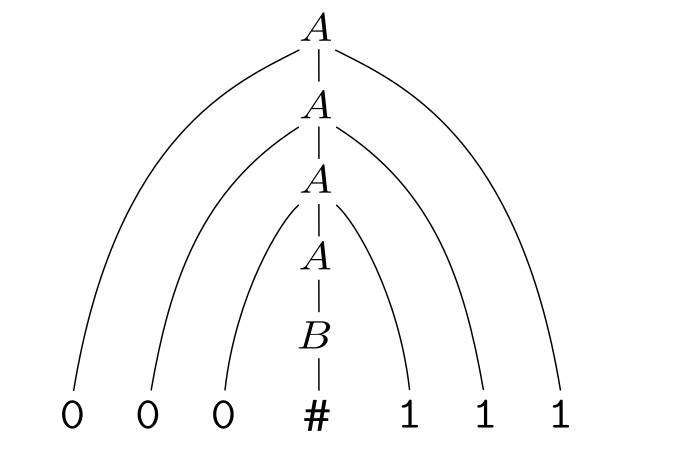
\includegraphics[scale=0.3]{figur/figur21.png}
	\end{center}
	\begin{itemize}
		\item Alle strenge der kan genereres fra \eqref{eq:cfgex} er dele af \textit{sproget af grammatikken}, som skrives $L(G_{1})$.
		\item \textbf{Ethvert sprog der kan genereres af en CFG er et kontekstfrit sprog}. (Definition, ikke sætning.)
	\end{itemize}
\end{frame}

\begin{frame}
	\frametitle{Formel Definition af Kontekstfri Grammatik}
	\begin{definition}[Kontekstfri Grammatik]
		En kontekstfri grammatik er en 4-tuple $(V, \Sigma, R, S)$, hvor
		\begin{enumerate}
			\item $V$ er en endelig mængde kaldet \textit{variabler}
			\item $\Sigma$ er en endelig mængde disjunkt fra $V$, kaldet \textit{terminaler}
			\item $R$ er en endelig mængde af \textit{regler}, hvor hver regel er en variabel (venstresiden) og en streng af variabler og terminaler (på højresiden)
			\item $S \in V$ er startvariablen
		\end{enumerate}
	\end{definition}
\end{frame}

\begin{frame}
	\frametitle{Kontekstfrie grammatikker, fortsat}

	\begin{itemize}
		\item Hvis $uAw$ kan blive til $uwv$, siger vi at $uAv$ \textit{giver} $uwv$, og skriver det $uAv \Rightarrow uwv$.
		\item Vi siger at $u$ \textit{udleder} (ikke afleder!) $v$ hvis der eksisterer en udledning $u \Rightarrow u_{1} \Rightarrow u_{2} \Rightarrow \cdots \Rightarrow u_{k} \Rightarrow v$.
		      \begin{itemize}
			      \item Vi skriver dette $u \overset{*}{\Rightarrow} v$ hvis $u = v$
		      \end{itemize}
		\item Sproget af en grammatik er dermed $\{w \in \Sigma^{*} \mid S \overset{*}{\Rightarrow}\}$
	\end{itemize}
\end{frame}

\begin{frame}[allowframebreaks]
	\frametitle{Tvetydighed}

	\begin{itemize}
		\item Hvis en grammatik kan generere den samme streng på mere end én forskellig måde, siger vi at strengen er afledt tvetydigt i den grammatik.
		\item Hvis en grammatik kan generere en streng tvetydigt, siger vi at selve grammatikken er \textit{tvetydig}.
	\end{itemize}

	\begin{equation}
		\langle \text{EXPR} \rangle \rightarrow \langle \text{EXPR} \rangle + \langle \text{EXPR} \rangle \mid \langle \text{EXPR} \rangle \times \langle \text{EXPR} \rangle \mid ( \langle \text{EXPR} \rangle ) \mid a
	\end{equation}

	\begin{itemize}
		\item Den ovenstående grammatik er tvetydig, da den generer strengen $a+a \times a$ tvetydigt.
		\item Vi kan se dette ved at lave to forskellige parsetræer:
	\end{itemize}

	\begin{center}
		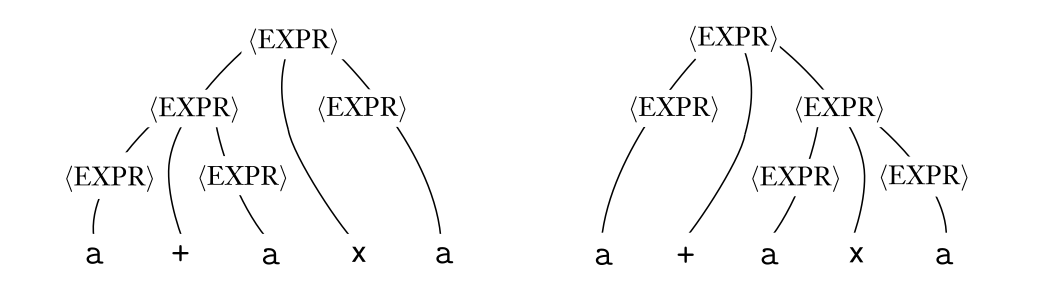
\includegraphics[scale=0.3]{figur/figur26.png}
	\end{center}
	\begin{itemize}
		\item Der eksisterer sproge der kun kan genereres af tvetydige grammatikker.
		\item Disse sprog siges at være \textit{i sig selv tvetydige}.
	\end{itemize}
\end{frame}

\begin{frame}[allowframebreaks]
	\frametitle{Chomsky Normal Form}

	\begin{itemize}
		\item (også kaldt, af Jørgen, Chomsky grammar).
		\item Chomsky Normal Form er en speciel \textit{form} til kontekstfrie grammatikker.
		\item Chomsky Normal Form sikrer nogle specifikke ting, der gør den brugbar til f.eks. algoritmer og beviser.
	\end{itemize}

	\begin{definition}[Chomsky Normal Form]
		En kontekstfri grammatik er i CNF hvis hver regel er af formen
		\begin{align*}
			A & \rightarrow BC \\
			A & \rightarrow a
		\end{align*}
		hvor $a$ er en vilkårlig terminal, og $A, B$ og $C$ er variabler, undtagen at $B$ og $C$ \textit{ikke} må være startvariablen. Vi tillader deruover også reglen $S \rightarrow \varepsilon$, hvor $S$ er startvariablen.
	\end{definition}

	\begin{theorem}
		Ethvert kontekstfrit sprog er genereret af en kontekstfri grammatik i CNF.
	\end{theorem}

	\begin{itemize}
		\item Vi kan konvertere en grammatik $G$ til CNF.
		\item Vi kan gøre dette ved at, trinvist, fjerne regler der ikke overholder betingelserne, og erstatter med regler der overholder.
		\item Først tilføjer vi en ny startvariabel.
		\item Så fjerner vi alle $\varepsilon$-regler af formen $A \rightarrow \varepsilon$.
		\item Vi eliminerer også alle \textit{unit regler} af formen $A\rightarrow B$.
		\item Til sidst konverterer vi de resterende regler til den rigtige form.
		\item \textbf{Bevis:}
	\end{itemize}
	\begin{enumerate}
		\item Først laver vi en ny startvariabel $S_{0}$, og tilføjer reglen $S_{0} \rightarrow S$, hvor $S$ var den tidligere variabel. Dermed sikrer vi at startvariablen ikke er på højresiden.
		\item Derefter tager vi os af epsilon-reglerne. Vi fjerner alle regler $A \rightarrow \varepsilon$ hvor $A$ ikke er starvariablen. \\ Derefter, for hver $A$ på højresiden af en regel, tilføjer vi en ny regel hvor vi fjerner $A$. Altså hvis $R \rightarrow uAv$ er en regel, tilføjer vi reglen $R \rightarrow uv$. Vi gørt dette for hvert tilfælde af $A$, så $R \rightarrow uavAw$ giver us tre regler: $R \rightarrow uvAw, R \rightarrow uAvw$ og $R \rightarrow uvw$. \\ Hvis reglen $R \rightarrow A$ eksisterer, erstatter vi denne med $R\rightarrow \varepsilon$, undtagen hvis $R \rightarrow \varepsilon$ er en regel vi allerede har fjernet. \\ Vi gentager dette indtil vi har fjernet alle epsilon-regler.
		\item Derefter fjerner vi alle \textit{unit regler}, altså for hvert $A \rightarrow B$ fjerner vi denne, og for alle $B \rightarrow u$, tilføjer vi $A \rightarrow u$, undtagen hvis dette er en regel vi allerede har fjernet, hvor $u$ er en streng af terminale og variabler. Vi gentager indtil alle unit regler er fjernet.
		\item Sidst konverterer vi alle tilbagestående regler til den rigtige form. For hvert $A \rightarrow u_{1}u_{2} \ldots u_{k}, k \ge 3$ fjerner vi denne regel, og tilføjer reglerne $A \rightarrow u_{1}A_{1}$, $A_{1} \rightarrow u_{2}A_{2}$, $A_{2} \rightarrow u_{3}A_{3}, \ldots A_{k-2} \rightarrow u_{k-1}u_{k}$
	\end{enumerate}
\end{frame}

\begin{frame}
	\frametitle{CFG Konverting Eksempel}
	Vi kigger på eksempel 2.10 pp. 110 i bogen for bedring af forståelse.
\end{frame}

\subsection{Pushdown Automater}%
\label{subsec:pda}


\begin{frame}[allowframebreaks]
	\frametitle{Pushdown Automater}
	\begin{itemize}
		\item Pushdown Automater (PDA) er ligesom NFA'er, men med en tilsluttet stak.
		\item Denne stak tillader pushdown automater at genkende flere sprog end en normal endelig automat, da den giver en uendelig hukommelse.
		\item Overførselsfunktionen for en PDA tillader dermed også \textit{pushing} og \textit{popping} af stakken.
		\item Stakken fungerer LIFO, og har dermed begrænset hukommelse.
		\item Sproget $\{0^{n}1^{n} \mid n \ge 0\}$ er et eksempel på et sprog der kan genkendes når vi nu har en stak:
		      \begin{itemize}
			      \item For hvert \texttt{0} der er læst, push det til stakken.
			      \item Når et \texttt{1} læses, pop for hvert 1 der er læst.
			      \item Hvis stakken er tom når der ikke er flere \texttt{1}'ere, så \textit{accepter}, ellers \textit{afvis}.
		      \end{itemize}

		\item En PDA er nondeterministisk, og er \textit{ikke} ækvivalent i sin deskriptive kraft til deterministiske automater med en stak. Disse genkender færre sprog.
	\end{itemize}
\end{frame}

\begin{frame}[allowframebreaks]
	\frametitle{Formel Definition af en Pushdown Automat}
	\begin{itemize}
		\item Det er ikke nødvendigt at bruge samme alfabet til input og til stak, dermed lader vi inputalfabetet være $\Sigma$ og stakalfabetet være $\Gamma$.
		\item Dermed er overførselsfunktionens domæne $Q \times \Sigma_{\varepsilon} \times \Gamma_{\varepsilon}$.
		\item Værdimængden fungerer som typisk ved nondeterminisme, men inklusiv stakken, da den også kan ændres. Dermed bliver værdimængden $\mathcal{P}(Q \times \Gamma_{\varepsilon})$.
	\end{itemize}

	\begin{definition}[Pushdown Automat]
		En \textit{pushdown automat} er en 6-tuple ($Q, \Sigma, \Gamma, \delta, q_{0}, F$), hvor $Q, \Sigma, \Gamma$ og $F$ alle er endelige mængder, og
		\begin{enumerate}
			\item $Q$ er mængden af tilstande
			\item $\Sigma$ er inputalfabetet
			\item $\Gamma$ er stakalfabetet
			\item $\delta : Q \times \Sigma_{\varepsilon} \times \Gamma_{\varepsilon} \longrightarrow \mathcal{P}(Q \times \Gamma_{\varepsilon})$ er overførselsfunktionen
			\item $q_{0} \in Q$ er starttilstanden
			\item $F \subseteq Q$ er mængden af accepttilstande
		\end{enumerate}
	\end{definition}

	\begin{itemize}
		\item Komputeringen i en pushdown automat fungerer som følge:
		\item Lad input $w$ være et input der accepteres hvis $w$ kan skrives $w = w_{1}, \ldots, w_{n}, $, hvor $\forall w_{i} : w_{i} \in \Sigma_{\varepsilon}$.
		\item En sekvens af tilstande $r_{0}, r_{1}, \ldots, r_{m} \in Q$ og strengene $s_{0}, s_{1}, \ldots, s_{m} \in \Gamma^{*}$ eksisterer som opfylder følgende tre betingelser:
		      \begin{enumerate}
			      \item $r_{0} = q_{0}$ og $s_{0} = \varepsilon$
			      \item $i = 0, \ldots, m-1 : (r_{i+1}, b) \in \delta(r_{i}, w_{i+1}, a)$, hvor $s_{i} = at$ og $s_{i+1} = bt$, hvor $a,b \in \Gamma_{\varepsilon}$ og $t \in \Gamma^{*}$. I.e., bevæger $M$ sig ifølge tilstanden, stakken og det næste inputsymbol.
			      \item $r_{m} \in F$. Denne betingelse siger at en accepttilstand forekommer i inputtets slutning.
		      \end{enumerate}
	\end{itemize}
\end{frame}

\begin{frame}[allowframebreaks]
	\frametitle{Eksempel 2.14}

	\begin{itemize}
		\item Vi vil nu beskrive en PDA der genkender $\{0^{n}1^{n} \mid n \ge 0\}$.
		\item Lad $M_{1} = (Q, \Sigma, \Gamma, \delta, q_{1}, F)$, hvor
		      \begin{enumerate}
			      \item[$Q = $] $\{q_{1}, q_{2}, q_{3}, q_{4}\}$
			      \item[$\Sigma = $] $\{0, 1\}$
			      \item[$\Gamma = $] $\{0, \mathdollar \}$
			      \item[$F = $] $\{q_{1}, q_{4}\}$
			      \item[$\delta = $]
			            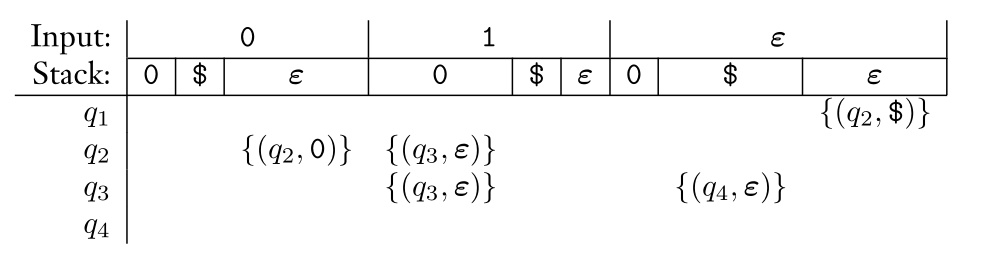
\includegraphics[scale=0.3]{figur/eksempel214.png}
		      \end{enumerate}

		\item Vi kan også lave en tilstandsdiagram. Bemærk her at $a,b \longrightarrow c$ betyder ``læs et $a$ fra input, erstat $b$ fra stakken med $c$'': \\
		      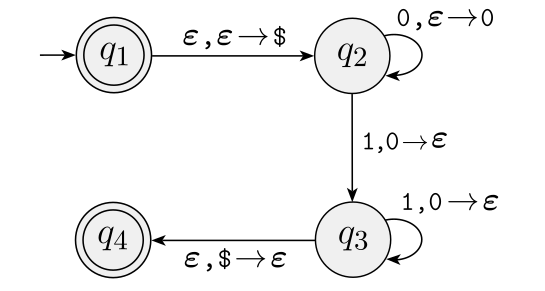
\includegraphics[scale=0.4]{figur/figur215.png}
	\end{itemize}
\end{frame}

\begin{frame}[allowframebreaks]
	\frametitle{Ækvivalens med Kontekstfrie Grammatikker}
	\begin{theorem}
		Et sprog er kontekstfrit hvis og kun hvis ($\iff$) en pushdown automat genkender det.
	\end{theorem}

	\begin{lemma}
		Hvis et sprog er kontekstfrit, så genkender en pushdown automat det.
	\end{lemma}

	\begin{itemize}
		\item Vi gør ligesom i bogen og kommer først med idéen, og derefter selve beviset:
		\item Vores mål er at vise at en CFG $G$ der genkender $A$ kan konverteres til en ækvivalent PDA $P$.
		\item PDA'en fungerer ved at acceptere input $w$ hvis $G$ genererer denne streng. Den finder ud af dette ved at finde ud af om der findes en afledning for $w$.
		\item Vi kalder en streng af variabler og terminaler der ikke er sluttet (afledt) og ikke er startstrengen for en \textit{mellemliggende streng} (intermediate string).
		\item Følgende er en uformel beskrivelse af PDA'en $P$:
		      \begin{enumerate}
			      \item Placer markeringssymbolet $\mathdollar$ og startvariablen på stakken
			      \item Gentag følgende skridt forevigt:
			            \begin{enumerate}
				            \item Hvis toppen af stakken er et variabelsymbol $A$, vælg nondeterministisk en af reglerne og erstat med højrehåndssiden.
				            \item Hvis toppen er et terminalsymbol, læs det næste symbol fra inputtet og sammenlign med $a$. Hvis de er lig hinanden, så gentag. Hvis ikke, så \textit{afvis} denne gren.
				            \item Hvis toppen af stakken er symbolet $\mathdollar$, gå til \textit{accepttilstanden}.
			            \end{enumerate}
		      \end{enumerate}

		\item Vi vil nu formalisere dette bevis.
		\item Lad $P = (Q, \Sigma, \Gamma, \delta, q_{start}, F)$ være en PDA.
		\item Vi laver en forsimplet notation til overførselsfunktionen:
		\item Lad $q$ og $r$ være tilstande i PDA'en, og lad $a \in \Sigma_{\varepsilon}, s \in \Gamma_{ \varepsilon}$.
		\item Vi vil gerne gå fra $q$ til $r$ når den læser $a$ og popper $s$.
		\item Derudover skal den pushe strengen $u = u_{1}, \ldots u_{l}$ til stakken på samme tid.
		\item Vi implmenterer denne handling ved at introducere nye tilstande $q_{1}, \ldots, q_{l-1}$, og lade overførselsfunktionen være som følger:
		      \begin{align*}
			       & \delta(q,a,s) \text{ indeholder } (q_{1}, u_{l}),              \\
			       & \delta(q_{1}, \varepsilon, \varepsilon) = \{(q_{2}, u_{l-1})\} \\
			       & \delta(q_{2}, \varepsilon, \varepsilon) = \{(q_{3}, u_{l-2})\} \\
			      \vdots                                                            \\
			       & \delta(q_{l-1}, \varepsilon, \varepsilon) = \{(r, u_{1})\}
		      \end{align*}

		\item Vi kan grafisk se implementering her:
		      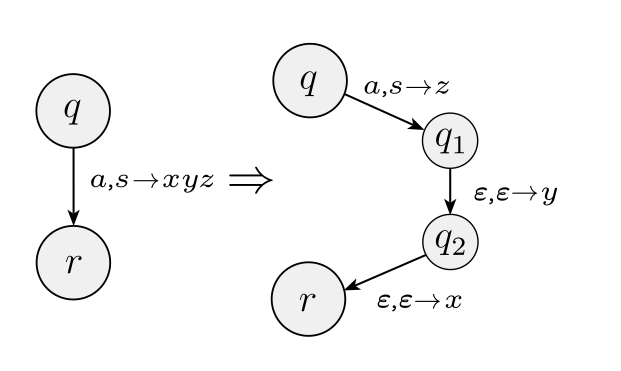
\includegraphics[scale=0.5]{figur/figur223.png}
		\item Tilstandene i $P$ er $Q = \{q_{start}, q_{gentag}, q_{accept}\} \cup E$ hvor $E$ er mængden af tilstandene vi skal bruge for at implementere \(\delta\). Ydermere $F = \{q_{accept}\}$.
		\item Vi definerer overførselsfunktionen som følger:
		      \begin{itemize}
			      \item Lad stakken starte med symbolerne $\mathdollar, S$. Det gør vi ved at bruge vores notation, $\delta(q_{start}, \varepsilon, \varepsilon) = \{(q_{loop}, S \mathdollar)\}$
			      \item Som det næste skal vi håndtere toppen af stakken. Til dette er der tre muligheder:
			            \begin{enumerate}
				            \item Toppen af stakken er en variabel\\ Lad $\delta(q_{loop}, \varepsilon, A) = \{(q_{loop}, w) \mid \text{ hvor } A \rightarrow w \text{ er en regel i }R\}$
				            \item Toppen af stakken er en terminal\\ Lad $\delta(q_{loop}, a, a) = \{(q_{loop}, \varepsilon)\}$
				            \item Toppen af stakken er tom (\textdollar) \\ Lad $\delta(q_{loop}, \varepsilon, \mathdollar) = \{(q_{accept}, \varepsilon)\}$
			            \end{enumerate}
		      \end{itemize}

		\item Vi kan se dette grafisk om følger:

		      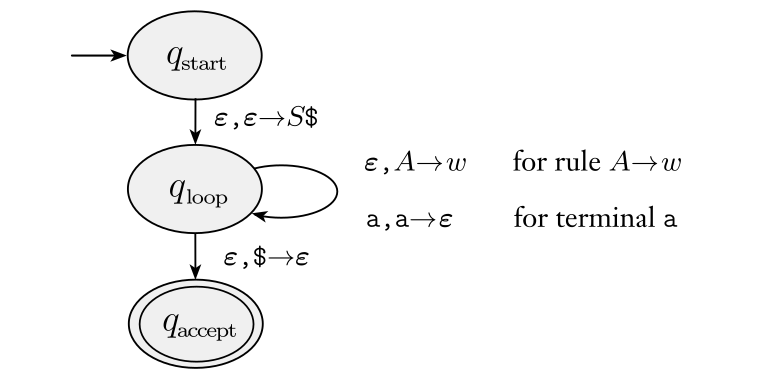
\includegraphics[scale=0.3]{figur/figur224.png}
	\end{itemize}
\end{frame}

\begin{frame}[allowframebreaks]
	\frametitle{Eksempel 2.25}

	\begin{itemize}
		\item Vi kigger hurtigt på et eksempel. Vi konstruerer en PDA fra CFG'en $G$:
	\end{itemize}
	\begin{align*}
		S & \rightarrow aTb \mid b          \\
		T & \rightarrow Ta \mid \varepsilon
	\end{align*}

	\begin{itemize}
		\item Overførselsfunktionen (samt hele tilstandsdaigrammet) kan ses i følgende diagram:
	\end{itemize}
	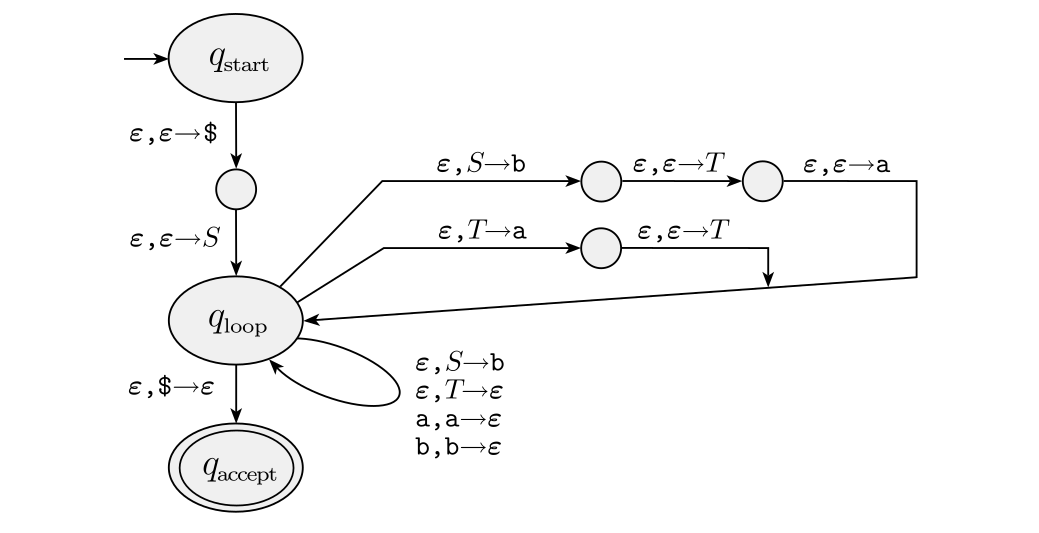
\includegraphics[scale=0.3]{figur/figur226.png}
\end{frame}

\begin{frame}[allowframebreaks]
	\frametitle{Ækvivalens Med Kontekstfrie Grammatikker 2}
	\begin{itemize}
		\item Vi vil nu bevise den anden retning.
	\end{itemize}

	\begin{lemma}
		Hvis en PDA genkender et sprog, så er det kontekst-frit.
	\end{lemma}

	\begin{itemize}
		\item Givet en PDA $P$, og en CFG $G$:
		\item For hvert par af states, $p$ og $q$ i $P$, vil vi have en variabel i grammatikken $A_{pq}$.
		\item Formålet med denne variabel er at den skal kunne generere alle strenge som kan tage $P$ fra $p$ med en tom stak til $q$ med en tom stak. Dette vil også betyde at stakken ikke ændrer sig overhovedet.
		\item Vi starter med at ændre lidt i $P$:
		      \begin{enumerate}
			      \item Den har én accept state $q_{accept}$
			      \item Den tømmer sin stak før den accepterer
			      \item Hver overførsel pusher enten et symbol til stakken eller popper et symbol fra stakken. Men ingen på samme tid.
		      \end{enumerate}
		\item Det er nemt at ændre i $P$ for at få den ønskede funktionalitet.
		\item For den 3. ændrer vi hver overførsel som både popper og pusher med to overførsler.
		\item Hver overførsel der hverken pusher eller popper, ændrer vi til to, hhv. en der først pusher og en der så popper.
		\item Vi ved at ved at gå fra en state $p$ til $q$ i PDA'en, givet en streng $x$, skal der \textit{pushes} før der kan \textit{poppes}. Vi ved dette præcis fordi vi antager at stakken er tom, eller at den i det mindste ikke ændrer på stakken. Dermed på der ikke poppes noget.
		\item Der er to muligheder, når $P$ kører på $x$:
		      \begin{enumerate}
			      \item Symbolet poppet i slutningen er symbolet pushet i starten.
			      \item Symbolet poppet i slutningen er \textit{ikke} symbolet pushet i starten.
		      \end{enumerate}

		\item Hvis (1) betyder det at stakken kun har været tom 2 gange: Før første push, og efter sidste pop.
		\item Hvis (2) må det første symbol blive poppet på et eller andet tidspunkt før $x$ er færdigkomputeret.
		\item Ved (1) kan vi simulere dette med reglen $A_{pq} \rightarrow aA_{rs}b$ hvor:
		      \begin{itemize}
			      \item $a$ er inputtet læst ved første overførsel
			      \item $b$ er inputtet læst ved sidste overførsel
			      \item $r$ er tilstanden efterfølgende $p$, og $s$ er tilstanden før $q$
		      \end{itemize}
		\item Ved (2) kan vi simulere den med reglen $A_{pq} \rightarrow A_{pr}A_{rq}$, hvor $r$ er tilstanden når stakken bliver tom.

		\item Visuelt forklaring for (1): 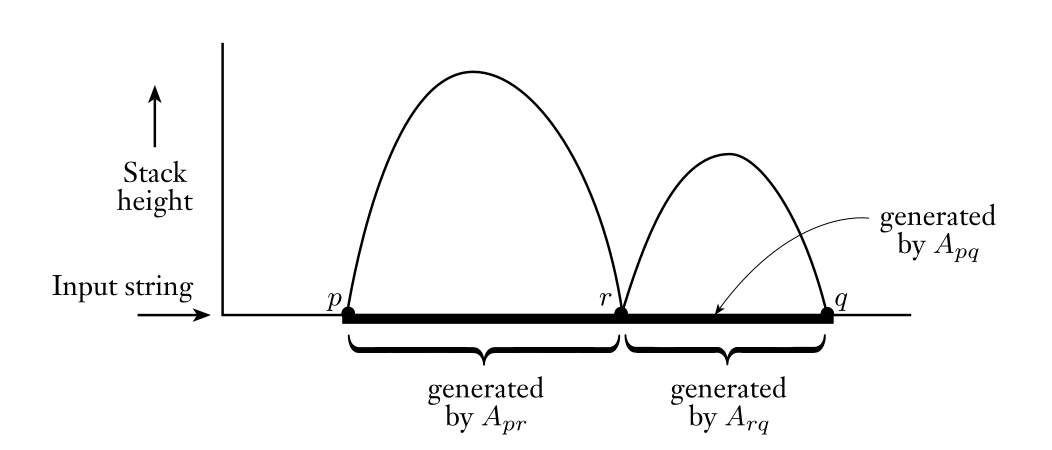
\includegraphics[scale=0.3]{figur/figur228.png}
		\item Visuelt forklaring for (2): 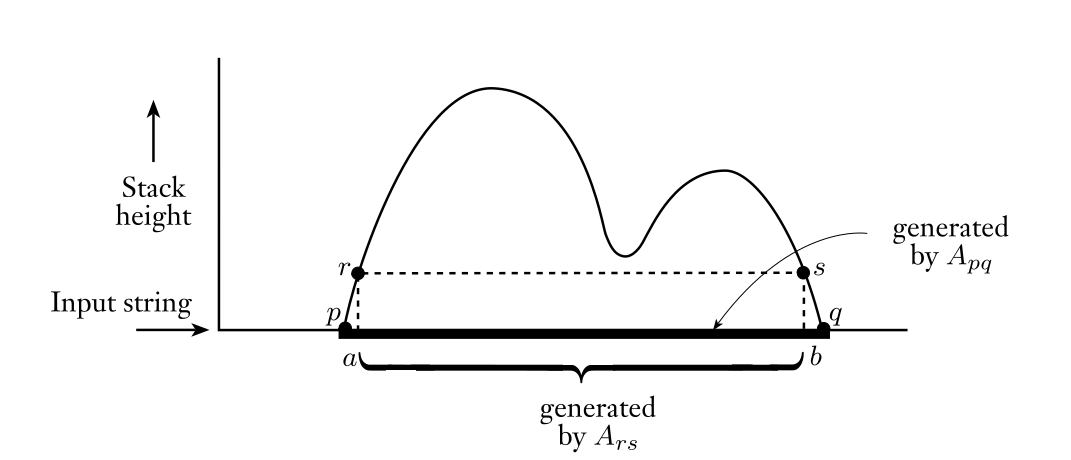
\includegraphics[scale=0.3]{figur/figur229.png}

		\item Nu til det formelle bevis (piv :( )
		\item Lad $P = (Q, \Sigma, \Gamma, \delta, q_{0}, \{q_{accept}\})$ og konstruer $G$.
		\item Variablerne af $G$ er $\{A_{pq} \mid p,q \in Q\}$
		\item Startvariablen er $A_{q_{0}, q_{accept}}$
		\item Vi beskriver $G$'s regler i tre dele:
		      \begin{enumerate}
			      \item For hvert $p,q,r,s \in Q, u \in \Gamma$ og $a,b \in \Sigma_{\varepsilon}$, hvis $\delta(p,a,\varepsilon)$ indeholder $(r,u)$ og $\delta(s,b,u)$ indeholder $(q, \varepsilon)$, put reglen $A_{pq} \rightarrow aA_{rs}b$ i $G$.
			      \item For hvert $p,q,r \in Q$, put reglen $A_{pq} \rightarrow A_{pr}A_{rq}$ i $G$
			      \item For hvert $p \in Q$, put reglen $A_{pp} \rightarrow \varepsilon$ i $G$
		      \end{enumerate}

		\item \textbf{Påstand}:
		      Hvis $A_{pq}$ genererer $x$, så kan $x$ bringe $P$ fra $p$ på en tom stak til $q$ med en tom stak.
		\item Vi beviser ved induktion.
		\item \textit{Basis}: Afledningen har ét skridt. Dette er trivielt bevist ved vores regel $A_{pp} \rightarrow \varepsilon$.
		\item \textit{Induktionsskridt}: Vi antager at det er sandt for afledninger af længde højest $k$, hvor $k \ge 1$, og beviser at det også gælder afledninger af længde $k+1$:
		\item Antag at $A_{pq} \overset{*}{\Rightarrow} x$ på $k+1$ skridt.
		\item Det første skridt i den afledning er enten $A_{pq} \Rightarrow aA_{rs}b$ eller $A_{pq} \Rightarrow A_{pr}A_{rq}$. Vi håndterer de to tilfælde seperat.
		\item I første tilfælde, lad os tænke på strengen i henhold til $y$, således at vi kan opdele $x$ til at være $x = ayb$, hvor $a$ og $b$ kender vi allerede.
		\item Fordi $A_{rs} \overset{*}{\Rightarrow} y$ med $k$ skridt, siger induktionshypotesen at $P$ kan gå fra $r$ på en tom stak til $s$ på en tom stak.
		\item Fordi $A_{pq} \rightarrow aA_{rs}b$ er en regel af $G$, indeholder $\delta(p,a,\varepsilon)$ $(r,u)$ og $\delta(s,b,u)$ indeholder $(q, \varepsilon)$, for et staksymbol $u$.
		\item Dermed, hvis $P$ starter på $p$ med en tom stak, efter at have læst $a$ kan den gå til tilstand $r$ og pushe $u$ til stakken.
		\item Så kan den læse strengen $y$ og bringe den til $s$ og lade $u$ være på stakken.
		\item Dermed, efter at have læst $b$ kan den gå til tilstand $q$ og poppe $u$ af stakken.
		\item Så $x$ kan gå fra $p$ på en tom stak til $q$ på en tom stak.
		\item I det andet tilfælde, antag at portionerne $y$ og $z$ af $x$  som $A_{pr}$ og $A_{rq}$ hhv. genererer, så $x = yz$.
		\item Fordi $A_{pr} \overset{*}{\Rightarrow} y$ på højest $k$ skridt og $A_{rq} \overset{*}{\Rightarrow} z$ på højest $k$ skridt, siger induktionshypotesen at $y$ kan bringe $P$ fra $p$ til $r$ og $z$ kan bringe $P$ fra $r$ til $q$ med en tom stak fra begyndelsen til slutningen. Dermed kan $x$ bringe den fra $p$ på en tom stak til $q$ med en tom stak.
		\item \textbf{Påstand}: Hvis $x$ kan bringe $P$ fra $p$ på en tom stak til $q$ på en tom stak, genererer $A_{pq}$ strengen $x$.
		\item Vi beviser igen ved induktion :)
		\item \textit{Basisskridt}. Komputeringen har $0$ skridt. Hvis komputeringen har 0 skridt starter og ender den på samme tilstand, e.g. $p$. Vi skal altså vise at $A_{pp} \overset{*}{\Rightarrow} x$. På 0 skirdt kan $P$ ikke læse nogen karakterer, så $x = \varepsilon$. Ved konstruktion, har $G$ reglen $A_{pp} \rightarrow \varepsilon$.
		\item \textit{Induktionsskridt}: Antag sand for komputationer af længde højest $k$, hvor $k \ge 0$, og bevis for $k+1$:
		\item Antag at $P$ har en komputering hvor $x$ bringer $p$ til $q$ på en tom stak i $k+1$ skridt.
		\item Så er stakken enten kun tom i begyndelsen og slutningen, eller den bliver tom på en eller flere tidspunkter mellem disse to.
		\item I første tilfælde (kun tom to gange) er symbolet der puishes i første overførsel det samme som symbolet der poppes i sidste overførsel.
		\item Vi kalder dette symbol $u$.
		\item Lad $a$ være inputtet læst i første overførsel og $b$ inputtet i sidste overførsel.
		\item Lad $r$ være tilstanden efter første overførsel, og $s$ tilstanden før sidste.
		\item Med det vil $\delta(p,a,\varepsilon)$ indeholde $(r,u)$ og $\delta(s,b,u)$ vil indeholder $(q,\varepsilon)$.
		\item Dermed er reglen $A_{pq} \rightarrow aA_{rs}b$ i $G$
		\item Lad $y$ være portionen af $x$ uden $a$ eller $b$, så $x = ayb$.
		\item Input $y$ kan bringe $P$ fra $r$ til $s$ på en tom stak uden at røre symbolet $u$ som er på styakken.
		\item Vi har fjernet første og sidste skridt af de $k+1$ skridt i den originale komputering af $x$, så komputeringen på $y$ har $(k+1)-2 = k-1$ skridt.
		\item Dermed siger induktionshypotesen at $A_{rs} \overset{*}{\Rightarrow} y$. Dermed $A_{pq} \overset{*}{\Rightarrow} x$.
		\item I andet tilfælde (3 eller flere gange der er en tom stak):
		\item Lad $r$ være en tilstand hvor stakken bliver tom andet end i begyndelsen eller slutningen af komputeringen på $x$.
		\item Så indeholder portionen af komputeringen fra $p$ til $r$ og fra $r$ til $q$ højest $k$ skridt.
		\item Hvis $y$ er inputet læst i første portion og $z$ i anden, så siger induktionshypotesen at $A_{pr} \overset{*}{\Rightarrow} y$ og $A_{rq} \overset{*}{\Rightarrow} z$. Fordi reglen $A_{pq} \rightarrow A_{pr}A_{rq}$ er i $G$, $A_{pq} \overset{*}{\Rightarrow} x$.
	\end{itemize}
\end{frame}

\begin{frame}[allowframebreaks]
	\frametitle{Jørgens Noter}
	\begin{itemize}
		\item En pushdown-automat (PDA) er en ikke-deterministisk endelig automat med en stak, hvilket gør PDA'er mere kraftfulde end DFA'er og NFA'er.
		\item Hvis en PDA skal være deterministisk, mister den evnen til at genkende visse sprog. Dette sker ikke for endelige automater.
		\item Et vigtigt faktum uden bevis (se papiret under noter på hjemmesiden) er, at hvert kontekstfrit sprog over et ét-symbols alfabet også er regulært. Du skal kunne bruge dette faktum, men ikke bevise det.
		\item Der findes sprog, der ikke er kontekstfrie, og pumpesætningen kan bruges til at bevise dette ved modstrid. Et eksempel er $\{a^n b^n c^n \mid n \geq 0\}$.
		\item Hvert regulært sprog er kontekstfrit.
		\item Klassen af kontekstfrie sprog er ikke lukket under fællesmængde. Der findes kontekstfrie sprog $L_1$ og $L_2$, hvor $L_1 \cap L_2$ ikke er kontekstfrit. For eksempel, hvis $L_1 = \{a^i b^j c^k \mid i, j, k \geq 0 \text{ og } i = j\}$ og $L_2 = \{a^i b^j c^k \mid i, j, k \geq 0 \text{ og } j = k\}$, så er både $L_1$ og $L_2$ kontekstfrie, men $L_1 \cap L_2 = \{a^n b^n c^n \mid n \geq 0\}$, hvilket ikke er kontekstfrit.
		\item PDA'er er ækvivalente med kontekstfrie grammatikker. For enhver PDA $A$ kan man konstruere en grammatik $G$ sådan at $L(A) = L(G)$, og omvendt.
		\item Klassen af kontekstfrie sprog er lukket under foreningsmængde, sammenkædning og stjerne, men ikke under fællesmængde og komplement. Dette betyder ikke, at komplementet af et kontekstfrit sprog aldrig er kontekstfrit. For eksempel er både $\Sigma^*$ og dets komplement, den tomme mængde, kontekstfrie (også regulære). Ligeledes er $L = \{a^n b^n \mid n \geq 0\}$ og dets komplement kontekstfrie (men ikke regulære).
		\item Fællesmængde af et kontekstfrit sprog $L_1$ med et regulært sprog $L_2$ er kontekstfrit. Hvis vi har en PDA $M_1$ for $L_1$ over $\Sigma$ og en DFA $M_2$ for $L_2$, kan vi lave en PDA $M$ som simulerer $M_1$ og $M_2$ parallelt. Den nye PDA $M$ har par af tilstande $(q, p)$, hvor $q$ er den aktuelle tilstand af $M_1$ og $p$ den aktuelle tilstand af $M_2$. Når $M$ læser et symbol $a \in \Sigma$, opdaterer den både $M_1$'s tilstand og stak samt $M_2$'s tilstand. $M$ accepterer en streng $w$ hvis og kun hvis både $M_1$ accepterer $w$ (med tom stak) og $M_2$ accepterer $w$. Derfor er $L_1 \cap L_2$ kontekstfrit, da det accepteres af en PDA.
	\end{itemize}
\end{frame}






%%% mode: latex
%%% TeX-engine: xetex
%%% TeX-command-extra-options: "-shell-escape"
%%% TeX-master: "main"
%%% End:
